\section{Introducci\'on}
\subsection{Descripción}
Es una empresa multinacional dedicada a la fabricación y comercialización de luminarias, farolas, columnas y soportes, que ofrece soluciones de excelente calidad luminotécnica en Alumbrado Público, Áreas Verdes, Alumbrado Industrial, Alumbrado Interior, Alumbrado de Jardín, Iluminación con Sumergibles y Leds.

\subsection{Ubicación}
La empresa se encuentra ubicada en las afueras de la Ciudad de Buenos Aires, m\'as precisamente en el conurbano bonaerense en el kil\'ometro 37.5 del ramal Escobar de la Ruta Panamericana. A pesar de encontrarse a aproximadamente 
40 kil\'ometros de la Capital Federal, es relativamente f\'acil y r\'apido llegar hasta la f\'abrica.

\subsection{Historia}
En el año 1922 Industrias Electrotécnicas Puig (IEP) se especializaba en la fabricación de aparatos reflectores para alumbrado en la española ciudad de Barcelona.
En el año 1966 pasa a formar parte del Grupo Simon, un holding de empresas del mercado eléctrico español con visionaria expansión hacia a los cinco continentes.
A principios de la década del 90 adapta nuevamente su estructura y su imagen, empezando a conocérsela como IEP DE ILUMINACIÓN.
Es en el año 1998 que IEP DE ILUMINACIÓN llega a la Argentina, convirtiéndose en el lapso de 12 años en la principal responsable de la comercialización de luminarias para toda América del Sur. 
Como en todo proceso de expansión y desarrollo, el Grupo Simon fue incorporando nuevos centros de producción y filiales en Latinoamérica (Argentina, Brasil y México), en Europa (Francia, Reino Unido, Irlanda, Bélgica, Holanda, Noruega, Suiza, Polonia), en África (Marruecos y Egipto) y en Asia (China, India, Rusia, Turquía) para poder llegar con mayor rapidez y eficiencia operativa a todos sus mercados.
En la actualidad cuenta con 24 empresas coordinadas desde su sede central en Barcelona (España) y su presencia mundial alcanza a más de 50 países. Centra sus actividades en el ámbito de la instalación eléctrica con diversas líneas de productos: material eléctrico y protección de circuitos, iluminación, domótica, conexiones para voz y datos, canalizaciones y electrónica. Las más recientes incorporaciones en su línea de negocios comprenden el mobiliario urbano y la seguridad. El primero por su relación con los espacios de iluminación urbana y el segundo porque las innovaciones aplicadas en este campo también incluyen material eléctrico.

\subsubsection{En Argentina}
Durante sus primeros años de actividad en el país, la empresa contó con planta de producción en la localidad de Munro (Buenos Aires) y oficinas comerciales en San Isidro (Buenos Aires), pero el creciente aumento de los volúmenes de venta fundados en la producción de luminarias de avanzada tecnología y diseños de vanguardia, demandó la instalación de una planta fabril de mayor tamaño y capacidad productiva.
Así, posicionada en el ámbito local como la empresa “Líder en Innovación Tecnológica”, IEP DE ILUMINACIÓN cuenta desde el año 2005 con instalaciones propias dentro del Centro Industrial Garín (Buenos Aires), garantizando rapidez operativa y de organización al reunir en un mismo lugar tanto sus áreas Comerciales como las de Producción y Almacenamiento.

\section{Filosof\'ia de la empresa}

\subsection{Misi\'on}

La misi\'on de la empresa consiste en operar un sistema rentable que les permita satisfacer las necesidades actuales y potenciales del mercado luminot\'ecnico, 
ofreciendo productos y servicios con verdadero valor agregado, a fin de construir relaciones fuertes y a largo plazo.

\subsection{Visi\'on}

La empresa define su visi\'on de la siguiente forma:\\
Ser considerada la empresa de iluminaci\'on m\'as pujante convirtiendonos en el proveedor preferido por el mercado luminot\'ecnico al ofrecer los mejores 
productos y servicios del rubro.
 
\subsection{Valores Corporativos}
La empresa enuncia sus valores de la siguiente manera: \\
Son los que guían nuestro diario desafío de construir relaciones fuertes y largo plazo:
\begin{itemize}
	\item Compromiso
	\item Respeto
	\item Cumplimiento
	\item Confiabilidad
	\item Innovación
	\item Colaboración
	\item Agilidad
\end{itemize}


\section{Estructura de la empresa}

\subsection{Organigrama}
A continuación se presenta el organigrama completo de la empresa. Ver imagen \ref{organigramaIEP}

\begin{figure}
  \centering
  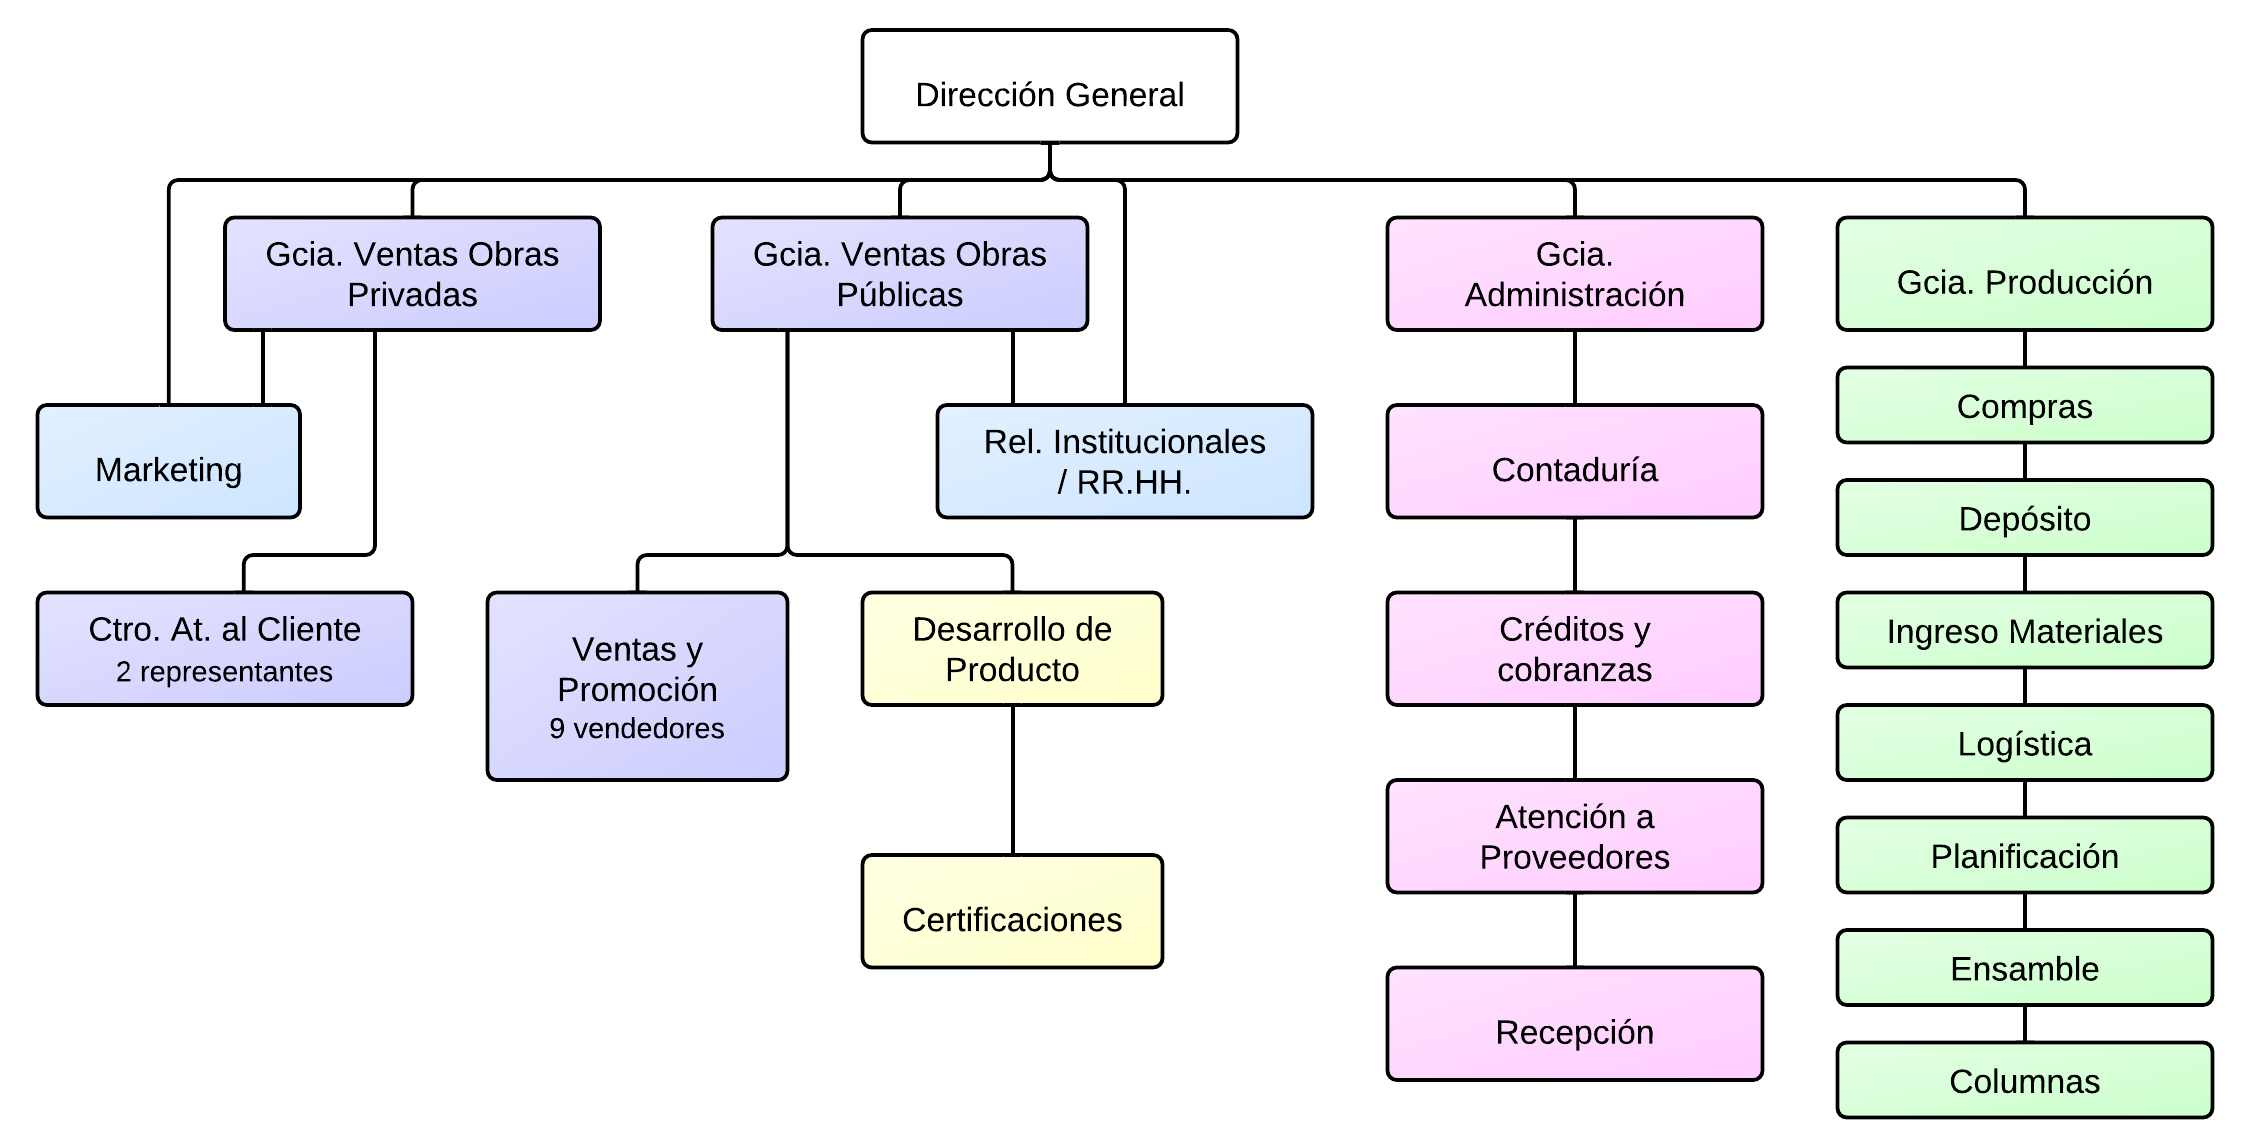
\includegraphics[scale=0.85]{./Images/organigrama-pasado.png}
  \caption{Organigrama IEP}\label{organigramaIEP}
\end{figure}

En la planta de Escobar se desempe\~nan cinco gerencias: Venta a Obras Privadas, Venta a Obras P\'ublicas, Administraci\'on, RR.HH. y Producci\'on. \\
El \'area m\'as importante es la de Producci\'on, pero la de Venta a Obras P\'ublicas tambi\'en involucra buena parte del personal de la planta. Este \'area cuenta con un Departamento de Desarrollo de Productos donde se dise\~nan y certifican productos a medida ofrecidos a dependencias p\'ublicas del \'ambito local.

\section{Productos que ofrece}
A grandes rasgos se trata de una empresa dedicada a la fabricaci\'on y comercializaci\'on de luminarias, farolas, columnas y soportes; ofreciendo soluciones de buena calidad en Alumbrado P\'ublico, \'Areas Verdes, Alumbrado Industrial, Alumbrado Interior, e incluso en Iluminaci\'on con Sumergibles y Leds.

\section{Sus clientes}
Los clientes principales de la empresa son los gobiernos municipales y provinciales de todo el territorio nacional.

Tambi\'en realizan ventan a barrios y urbanizaciones privadas y, en menor medida, a plantas industriales y cooperativas de vialidad.

\section{Sistemas de Informaci\'on}

IEP de Iluminaci\'on utiliza para la sistematizaci\'on de sus procesos un sistema integral de ERP de la empresa argentina Sistemas Bejerman, denominado eFlex.

Utilizan gran parte de los m\'odulos disponibles:

\begin{itemize}
\item Ventas y cuentas a cobrar
\item Compras y cuentas a pagar
\item Finanzas
\item Producci\'on
\item Contabilidad
\item Impuestos
\item CRM
\item Queries (Reportes)
\end{itemize}

\section{ Circuitos de Informaci\'on}
\subsection{ Elecci\'on de los circuitos}

La empresa ha entregado un documento en el cual se encuentran descriptos varios circuitos de informaci\'on. Varios de estos son muy particulares y especificos, por lo que a la hora de decidir que circuitos se van a documentar se procede a agrupar algunos seg\'un conveniencia.
La seleccion de los mismos fue:
\begin{itemize}
\item Compra de materiales y entrada de inventario.
\item Pedido de ventas con transporte propio.
\item Cobro de facturas
\end{itemize}

La elecci\'on de los mismos fue basada en la cantidad y calidad de la informaci\'on que se poseia de estos en relaci\'on a los que quedaron de lado. Es decir, se tienen en cuenta los documentos que los circuitos implican, la cantidad de los mismos y como es su relaci\'on con las distintas areas de la empresa.